%----------------------- Wydruk dwustronny ---------------
%\documentclass[12pt,twoside,a4paper]{book} % 
%----------------------- Wydruk jednostronny ---------------
\documentclass[12pt,oneside,a4paper]{book} % jednostronnego

\usepackage{polski}
\usepackage[utf8]{inputenc} %opcja dla edytorów kodujących polskie znaki w utf8
%\usepackage[cp1250]{inputenc} %opcja dla edytorów kodujących polskie znaki w windows-1250
\usepackage{lmodern}
\usepackage{indentfirst}
\usepackage[protrusion=false]{microtype}
\DisableLigatures{encoding = *, family = * }
\usepackage{fancyhdr}
\usepackage{pstricks,graphicx}
\usepackage{amssymb}
\usepackage{float}

\usepackage{pdflscape}
\usepackage{diagbox}

%---------------Zbiory liczbowe
\newcommand{\R}{\mathbb{R}}
\newcommand{\N}{\mathbb{N}}
\newcommand{\K}{\mathbb{K}}
\newcommand{\C}{\mathcal{C}}
\newcommand{\p}{\mathcal{P}}
%------------kwantyfikatory--------------
\newcommand{\fal}{\mbox{{\Large $\forall\,$}}}
\newcommand{\ext}{\mbox{{\Large $\exists\,$}}}
%------------------definicje środowisk-----------------
\usepackage{theorem}
\theoremstyle{break}
\theorembodyfont{\it}
\newtheorem{twr}{Twierdzenie}[chapter]
\newtheorem{lem}{Lemat}[chapter]
\theorembodyfont{\rm}
\newtheorem{defi}{Definicja}[chapter]
\newtheorem{wni}{Wniosek}[chapter]
\newtheorem{prz}{Przykład}[chapter]
\newenvironment{dowod}{\par\vspace{0.1cm}\par{ \sc Dowód.}}{\hfill $\blacksquare$\par\vspace{0.4cm}\par}
% ----------ustawienia wymiarow strony
\usepackage{geometry}

\newgeometry{tmargin=2.5cm, bmargin=2.5cm, headheight=14.5pt, inner=3cm, outer=2.5cm} 

\linespread{1.1} %-zmiana interlinii


\fancypagestyle{mylandscape}{
\fancyhf{} %Clears the header/footer
\fancyfoot{% Footer
\makebox[\textwidth][r]{% Right
  \rlap{\hspace{.75cm}% Push out of margin by \footskip
    \smash{% Remove vertical height
      \raisebox{4.87in}{% Raise vertically
        \rotatebox{90}{\thepage}}}}}}% Rotate counter-clockwise
\renewcommand{\headrulewidth}{0pt}% No header rule
\renewcommand{\footrulewidth}{0pt}% No footer rule
}

%---------------- Normalne środowiska --------------------
\usepackage{amsmath}

%----------nagłowki i żywa pagina ------------
\pagestyle{fancy} 
%--------------- Wydruk dwustronny
%\cfoot[]{} 
%\lhead[{\scriptsize{\it \thepage}}]{}
%\chead[{\scriptsize\leftmark}]{{\scriptsize \rightmark}}
%\rhead[]{{\scriptsize{\it \thepage}}}
%--------------- Wydruk jednostronny
\fancyhead[C]{} 
\fancyfoot[C]{\thepage}
\fancyhead[L]{\scriptsize\leftmark}
\fancyhead[R]{\scriptsize\rightmark}

\renewcommand{\chaptermark}[1]{%
\markboth{\MakeUppercase{%
\chaptername}\ \thechapter.%
\ #1}{}}

\usepackage[most]{tcolorbox}
\let\includegraphicsold\includegraphics
\newcommand{\includegraphicsborder}[2][]{\tcbox{\includegraphicsold[#1]{#2}}}

\renewcommand{\sectionmark}[1]{\markright{\thesection.\ #1}}

\usepackage[hidelinks]{hyperref}

\usepackage{graphics}
\graphicspath{ {images/} }

\usepackage{listings}

\renewcommand{\lstlistlistingname}{Spis listingów}
\renewcommand{\lstlistingname}{Listing}

\lstset{
  basicstyle=\footnotesize
}

\usepackage{booktabs}

\newcommand\tabularhead[2]{
  \begin{table}[ht]
    \label{#2}
    \caption{#1}
    \begin{tabular}{|p{0.35\linewidth}|p{0.6\linewidth}|}
    \hline
    \textbf{#1}\\
    \hline
}
\newcommand\addrow[2]{#1 &#2\\ \hline}

\newcommand\addmulrow[2]{ \begin{minipage}[t][][t]{2.5cm}#1\end{minipage}
   &\begin{minipage}[t][][t]{8cm}
    \begin{enumerate} #2   \end{enumerate}
    \end{minipage}\\ }

\newenvironment{usecase}{\tabularhead}
{\hline\end{tabular}\end{table}}



%-----------------właściwa część pracy-----------------
\begin{document}
\thispagestyle{empty}
\begin{center}
  \Large
  \bf{UNIWERSYTET ŚLĄSKI}\\
  \bf{\sf{WYDZIAŁ NAUK ŚCISŁYCH I TECHNICZNYCH}}\\[25mm]
  \large

  \bf{Klasyfikatory w Rapid Miner}\\[35mm]

  Sprawozdanie\\
  z przedmiotu\\
  Eksploracja Danych\\[25mm]
\end{center}
\begin{flushright}
  \large
  Autorzy:\\
  Kacper Małachowski\\
\end{flushright}
\vspace*{\fill}
\begin{center}
  Informatyka II Stopnia\\
  Lato 2023/2024\\
  I rok, grupa 3\\[25mm]
\end{center}

\chapter*{Źródło danych}

Dane pochodzą z repozytorium uniwersytetu kalifornijskiego, gdzie znajdują się pod nazwą "Room Occupancy Estimation".
Stworzone zostały w ramach badań: Adarsh Pal Singh, Vivek Jain, Sachin Chaudhari, Frank Alexander Kraemer, Stefan Werner and Vishal Garg, "Machine Learning-Based Occupancy Estimation Using Multivariate Sensor Nodes," in 2018 IEEE Globecom Workshops (GC Wkshps), 2018.

Dane wczytane w obecnym projekcie są danymi przygotowanymi w najlepszej ścieżce z projektu 1. W procesie przygotowania danych, usunięto brakujące wartosci z pomocą operatora "Replace Missing Values" zastępuje je wartościami minimalnymi oraz poddano dane dyskretyzacji po kolumnie "S1\_Light" (”attribute filter type” z wartoscią ”single” oraz ”attribute” z wartością ”S1 Light”) z domyślną wartością 10 atrybutu ”number of~bins”.

\subsection*{Opis atrybutów}

\begin{itemize}
  \item Date - Pominięty w eksploracji - Data pomiaru z czujników.
  \item Time - Pominięty w eksploracji - Czas pomiaru z czujników z dokładnością do sekund.
  \item S1\_Temp - Odczyt z czujnika temperatury umieszczonego przy biurku nr 1, podany w stopniach celsjusza.
  \item S2\_Temp - Odczyt z czujnika temperatury umieszczonego przy biurku nr 2, podany w stopniach celsjusza.
  \item S3\_Temp - Odczyt z czujnika temperatury umieszczonego przy biurku nr 3, podany w stopniach celsjusza.
  \item S4\_Temp - Odczyt z czujnika temperatury umieszczonego przy biurku nr 4, podany w stopniach celsjusza.
  \item S1\_Light - Odczyt z czujnika światła umieszczonego przy biurku nr 1, podany w~luxach.
  \item S2\_Light - Odczyt z czujnika światła umieszczonego przy biurku nr 2, podany w~luxach.
  \item S3\_Light - Odczyt z czujnika światła umieszczonego przy biurku nr 3, podany w~luxach.
  \item S4\_Light - Odczyt z czujnika światła umieszczonego przy biurku nr 4, podany w~luxach.
  \item S1\_Sound - Odczyt z przetwornika analogowo-cyfrowego podłączonego do wyjścia wzmacniacza mikrofonu, wyrażony w woltach. Czujnik ten umieszczony jest przy biurku nr 1.
  \item S2\_Sound - Odczyt z przetwornika analogowo-cyfrowego podłączonego do wyjścia wzmacniacza mikrofonu, wyrażony w woltach. Czujnik ten umieszczony jest przy biurku nr 2.
  \item S3\_Sound - Odczyt z przetwornika analogowo-cyfrowego podłączonego do wyjścia wzmacniacza mikrofonu, wyrażony w woltach. Czujnik ten umieszczony jest przy biurku nr 3.
  \item S4\_Sound - Odczyt z przetwornika analogowo-cyfrowego podłączonego do wyjścia wzmacniacza mikrofonu, wyrażony w woltach. Czujnik ten umieszczony jest przy biurku nr 4.
  \item S5\_CO2 - Odczyt z detektora CO2, umieszczonego na środku pokoju, wyrażony w~cząsteczkach na milion.
  \item S5\_CO2\_Slope - Zmiana stężenia CO2 w pomieszczeniu z detektora umieszczonego na środku pomieszczenia.
  \item S6\_PIR - Wartość prawda-fałsz wskazująca na wykrycie ruchu przez czujnik umieszczony nad drzwiami.
  \item S7\_PIR - Wartość prawda-fałsz wskazująca na wykrycie ruchu przez czujnik umieszczony na ścianie na przeciwko drzwi.
\end{itemize}

\chapter*{Projekt w Rapid Miner}

Ponizej przedstawiono zdjęcie projektu z programu Rapid Miner.

\begin{figure}[H]
  \centering
  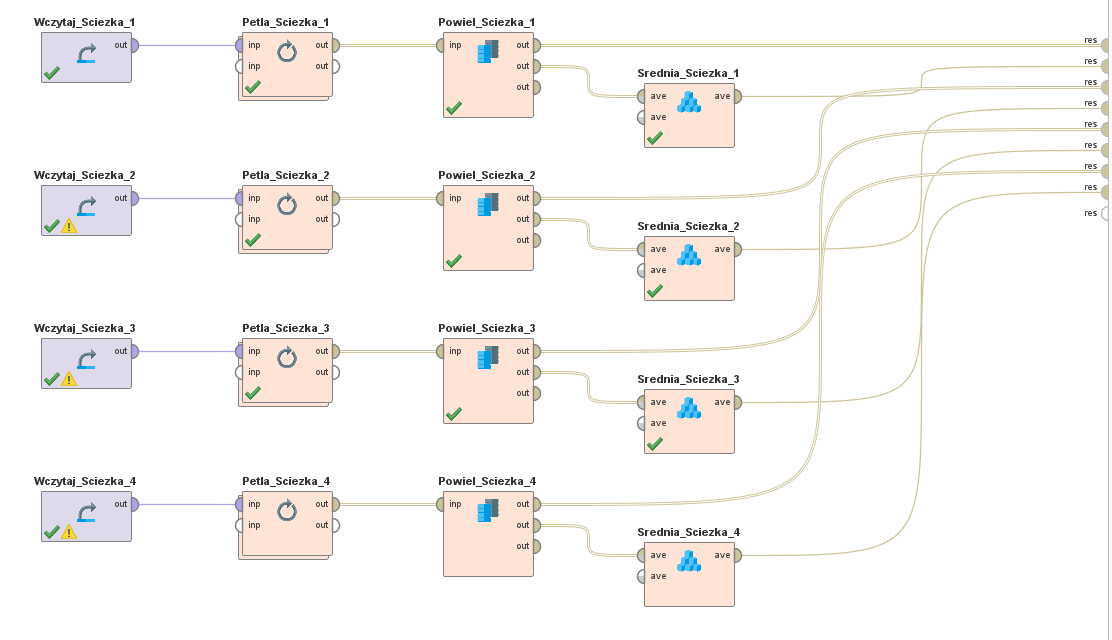
\includegraphics[width=1\textwidth]{project.png}
\end{figure}

\subsection*{Opis składowych projektu}

Projekt posiada kilka elementów wspólnych dla wszystkich ścieżek. Podstawowymi elementami są operatory Multiply oraz Average. Oba operatory nie posiadją atrybutów.

Kolejnym prostym operatorem jest Retrieve, który służy do wczytania danych z repozytorium. Parametr "repository entry" ustawiona na ścieżkę z danymi przygotowanymi w najlepszej ścieżce.

Pętle są również wspólne dla wszystkich ścieżek. Składają się one z umieszczonych wewnątrz walidacji krzyżowych, a parametry ścieżek prezentują się następująco.

\begin{itemize}
  \item number of iterations - liczba iteracji pętli - 20
  \item iteration macro - iteration
  \item reuse results - false
\end{itemize}

\newpage
Parametry krzyżowych walidacji wraz z sekcją testowania modeli są również wspólne dla wszystkich ścieżek. Parametry to:

\begin{itemize}
  \item leave one out - false
  \item number of folds - liczba podziałów - 10
  \item sampling type - automatic
\end{itemize}

Wewnątrz sekcji testującej wytrenowany model umieszczono operatory Apply Model oraz Performance, które nie posiadają atrybutów do ustawienia.

Następny element do omówienia to zastosowane modele w poszczególnych ścieżkach.

\subsubsection*{Ścieżka 1}

W pierwszej ścieżce zastosowano ten sam model, co w projekcie pierwszym, czyli Decision Tree.

Parametry tego modelu to:
\begin{itemize}
  \item criterion - gain\_ratio
  \item maximal depth - 10
  \item apply prunning - true
  \item confidence - 0.1
  \item apply preprunning - true
  \item minimal gain - 0.01
  \item minimal leaf size - 2
\end{itemize}

\subsubsection*{Ścieżka 2}

W drugiej ścieżce zastosowano model k-NN (k najblizszych sąsiadów). W ramach prób sprawdzono ustawienie innych wartości parametru k, jednak domyślna wartość 5 sprawdziła się najlepiej, spadek jakości następował w okolicach wartości k = 10.

\begin{itemize}
  \item k - 5
  \item weighted vote - true
  \item measure types - MixedMeasures
  \item mixed measure - MixedEuclideanDistance
\end{itemize}

\subsubsection*{Ścieżka 3}

W trzeciej ścieżce, użyto natomiast modelu naiwnego bayesa (Naive Bayes), który nie posiada żadnych parametrów do ustawienia.

\subsubsection*{Ścieżka 4}

W ścieżce czwartej zastosowano meta-klasyfikator Vote, który jest operatorem złożonym składającym się z użytych wcześniej modeli.
Sam operator Vote nie ma parametrów.

Jako pierwszy model od góry znajduje się Decision Tree, z parametrami:
\begin{itemize}
  \item criterion - gain\_ratio
  \item maximal depth - 10
  \item apply prunning - true
  \item confidence - 0.1
  \item apply preprunning - true
  \item minimal gain - 0.01
  \item minimal leaf size - 2
\end{itemize}

Drugim modelem jest użyty już w ścieżce 2 k-NN z parametrami:
\begin{itemize}
  \item k - 5
  \item weighted vote - true
  \item measure types - MixedMeasures
  \item mixed measure - MixedEuclideanDistance
\end{itemize}

Ostatnim modelem natomiast jest Naive Bayes, który nie posiada parametrów.

Wybór poszczególnych modeli, wraz z ustawieniem parametrów takich samych jak w ich ścieżkach podyktowany został chęcią sprawdzenia jak modele sprawdzą się przy założeniu głosowania między nimi.

\begin{landscape}
\thispagestyle{mylandscape}
\chapter*{Wyniki walidacji krzyżowej}

W poniższej tabeli przedstawiono wyniki walidacji krzyżowej dla poszczególnych ścieżek i iteracji pętli. Wyniki wyrażone są jako procent dokładności modelu.

\begin{table}[H]
  \resizebox{1.5\textwidth}{!}{
  \begin{tabular}{|c|c|c|c|c|c|c|c|c|c|c|c|c|c|c|c|c|c|c|c|c|c|c|}
  \hline
  \backslashbox{Ścieżka}{Iteracja}  & 1 & 2 & 3 & 4 & 5 & 6 & 7 & 8 & 9 & 10 & 11 & 12 & 13 & 14 & 15 & 16 & 17 & 18 & 19 & 20 & Średnia \\ \hline
   1  & 98.60\% & 98.56\% & 98.47\% & 98.67\% & 98.58\% & 98.82\% & 98.62\% & 98.48\% & 98.58\% & 98.60\% & 98.69\% & 98.57\% & 98.54\% & 98.48\% & 98.51\% & 98.61\% & 98.45\% & 98.55\% & 98.61\% & 98.50\% & 98.58\% \\ \hline
   2  & 99.54\% & 99.51\% & 99.55\% & 99.57\% & 99.55\% & 99.55\% & 99.52\% & 99.55\% & 99.55\% & 99.52\% & 99.53\% & 99.52\% & 99.52\% & 99.53\% & 99.53\% & 99.52\% & 99.54\% & 99.54\% & 99.58\% & 99.54\% & 99.53\% \\ \hline
   3  & 96.26\% & 96.15\% & 96.28\% & 96.28\% & 96.07\% & 96.18\% & 96.27\% & 96.15\% & 96.21\% & 96.21\% & 96.31\% & 96.29\% & 96.14\% & 96.18\% & 96.18\% & 96.15\% & 96.18\% & 96.21\% & 96.17\% & 96.16\% & 96.22\% \\ \hline
   4  & 99.26\% & 99.24\% & 99.30\% & 99.21\% & 99.31\% & 99.24\% & 99.25\% & 99.25\% & 99.27\% & 99.24\% & 99.24\% & 99.25\% & 99.21\% & 99.20\% & 99.31\% & 99.28\% & 99.23\% & 99.25\% & 99.30\% & 99.25\% & 99.26\% \\ \hline
  \end{tabular}}
  \end{table}

\end{landscape}

\chapter*{Wnioski}

Najlepiej z klasyfikacją danych poradził sobie model zbudowany w oparciu o~k~najblizszych sąsiadów. który uzyskał poprawę prawie o 1 punkt procentowy (dokładnie 0.95 punktu procentowego) uzyskując wynik, który statystycznie można potraktować jako dokładny: 99.53\%. 

Niestety połączenie klasyfikatorów poprzez głosowanie nie poprawiło wyników, w~sposób tak znaczący uzyskując jedynie dokładność klasyfikacji na poziomie 99.26\%.

Najgorszy wynik natomiast przedstawia model oparty o naiwnego bayesa. Nie tylko nie uzyskał on poprawy względem drzewa decyzyjnego, ale również znacząco obniżył jakość klasyfikacji.

Biorąc powyższe pod uwagę stwierdzić można, że wynik głosowania zaniżył algorytm naiwnego bayesa, jednak wymaga to dalszych badań w celu potwierdzenia tej hipotezy.
Bez wątpliwości pozostaje natomiast, że w przypadku tego zbioru danych najlepszy wynik daje zastowanie modelu opartego o algorytm k-NN poprzedzony dyskretyzacją.

Pozostałe 0.47 punktu procentowego dokładności można spokojnie uznać za statystyczny błąd, chociaż wyniki poszczególnych iteracji pokazują stabilność klasyfikacji w~tym przypadku.

\end{document}